%\documentclass[]{article}
%\usepackage{natbib}
\documentclass[extra,mreferee]{gji}
\usepackage{timet}
\usepackage{amsmath}
\usepackage{graphicx}
\usepackage[utf8]{inputenc}
\newcommand{\mbf}[1]{\mathbf{{#1}}}

\usepackage{todonotes}

% Document metadata
% =================
\newcommand{\Title}{
    Non-linear gravity inversion in spherical coordinates:
    application to the South American Moho
}
\newcommand{\Keywords}{
        Moho;
        gravity inversion;
        spherical coordinates;
        tesseroid;
        South America
}
\title[]{\Title}
\author[]{
    Leonardo Uieda$^{1,2}$,
    Valéria C. F. Barbosa$^{2}$
    \\
    $^1$Universidade do Estado do Rio de Janeiro, Rio de Janeiro, Brazil.
    e-mail: leo@leouieda.com
    \\
    $^2$Observatório Nacional, Rio de Janeiro, Brazil.
}

\usepackage[pdftex,colorlinks=true,hidelinks]{hyperref}
\hypersetup{
    pdftitle={\Title},
    pdfauthor={Leonardo Uieda (leo@leouieda.com)},
    pdfsubject={},
    pdfkeywords={\Keywords},
    pdfcreator={pdfTeX}
}



\begin{document}

%\label{firstpage}
\maketitle

\noindent \textbf{Keywords:} \Keywords

\begin{abstract}
\end{abstract}



%%%%%%%%%%%%%%%%%%%%%%%%%%%%%%%%%%%%%%%%%%%%%%%%%%%%%%%%%%%%%%%%%%%%%%%%%%%%%%%
\section{Introduction}


%%%%%%%%%%%%%%%%%%%%%%%%%%%%%%%%%%%%%%%%%%%%%%%%%%%%%%%%%%%%%%%%%%%%%%%%%%%%%%%
\section{Methodology}

We must first isolate the target anomalous density distribution.
In our case, the target is the relief of the real Moho undulating around a
reference Moho.
We do this by removing all other effects from the gravity observations.
The first correction is to remove the gravity\footnote{The term ``gravity''
refers the sum of the gravitational and centripetal accelerations.}
of an ellipsoidal Earth (the Normal Earth or reference ellipsoid).
This is done using the formula presented in \citet{li_ellipsoid_2001}.
The resulting quantity is known as the gravity disturbance,

\begin{equation}
    \delta g(P) = g(P) - \gamma(P)
\end{equation}

\noindent in which $g(P)$ is the measured gravity at an observation point $P$
and $\gamma(P)$ is the gravity of the Normal Earth (the Normal Gravity)
calculated on point $P$.

We assume that the crust of our Normal Earth has a standard density of
$\rho_{crust} = 2670\ kg.m^{-3}$ and depth $z_{ref}$.
The disturbance contains only the gravitational effects of density
distributions that are anomalous with respect to the Normal Earth.
This includes all masses above the surface of the ellipsoid (the topography),
the mass deficiency of the oceans,
the mass deficiency of sedimentary basins,
crustal sources (e.g., igneous intrusions, lateral density changes, etc),
heterogeneities below the upper mantle,
and
the mass excesses and deficiencies caused by differences between the real Moho
topography and the reference Moho ($z_{ref}$).
The last is what we are interested in.
All effects must either be removed or assumed negligible.
The input data for the inversion is assumed to be the isolated gravitational
effect of the anomalous Moho.



\subsection{Parametrization}


Assume all other sources were removed.
Only Moho topography around a reference level.
\todo{Include figure of Moho with all else  removed.}
Discretize into tesseroids.
Parameters are the Moho depths.
Establish that the reference level ($h_{ref}$)  and density contrast
($\Delta\rho_j$) are hyper-parameters.

\subsection{Inverse problem}

Formulate regularized inversion using Gauss-Newton and Steepest Descent.
Use full Jacobian.

\subsection{Bott's method}

Bott as Gauss-Newton.
Jacobian is diagonal.
Approximate the Jacobian by making tesseroid size tend to infinity to get
Bouguer slab.
This approximation is good for tesseroids because each will cover a large
enough area.
Show case for the Steepest Descent.
Extend the Jacobian to include lateral density variation.
Important because density-contrast is positive or negative depending if the
Moho is above or below the reference level.
Enforce that the use of a particular

Biggest computation time is in forward modeling.
All matrices involved are sparse.
Solve the sparse linear system with a conjugate gradient method.
\todo{Check which conjugate gradient scipy.space.linalg.solve uses.}
Use the regularized inversion because multiplying and solving the linear system
are fast compared to forward modeling.
Not using step size optimization because forward modeling is very slow so
increased convergence doesn't justify the extra time spent on the discarded
step attempts.

\subsection{Determination of hyper-parameters}



\subsection{Software implementation}

\todo{Cite packages in the references.txt file.}

\subsection{Satellite gravity data}


Explain where data came from and what was done to  it.


%%%%%%%%%%%%%%%%%%%%%%%%%%%%%%%%%%%%%%%%%%%%%%%%%%%%%%%%%%%%%%%%%%%%%%%%%%%%%%%
\section{Application to synthetic data from a simple model}


Meh.

%\begin{figure}
    %\centering
    %\includegraphics[width=\columnwidth]{figures/figure}
    %\caption{This is a figure caption.}
    %\label{fig:myfig}
%\end{figure}

%%%%%%%%%%%%%%%%%%%%%%%%%%%%%%%%%%%%%%%%%%%%%%%%%%%%%%%%%%%%%%%%%%%%%%%%%%%%%%%
\section{Application to synthetic data from the CRUST1.0 model}

Meh.


%%%%%%%%%%%%%%%%%%%%%%%%%%%%%%%%%%%%%%%%%%%%%%%%%%%%%%%%%%%%%%%%%%%%%%%%%%%%%%%
\section{Application to the South American Moho}

\begin{figure*}
    \centering
    \includegraphics[width=\textwidth]{figures/paper/sam-gravity-data}
    \caption{This is a figure caption.}
    \label{fig:sam-data}
\end{figure*}

\begin{figure*}
    \centering
    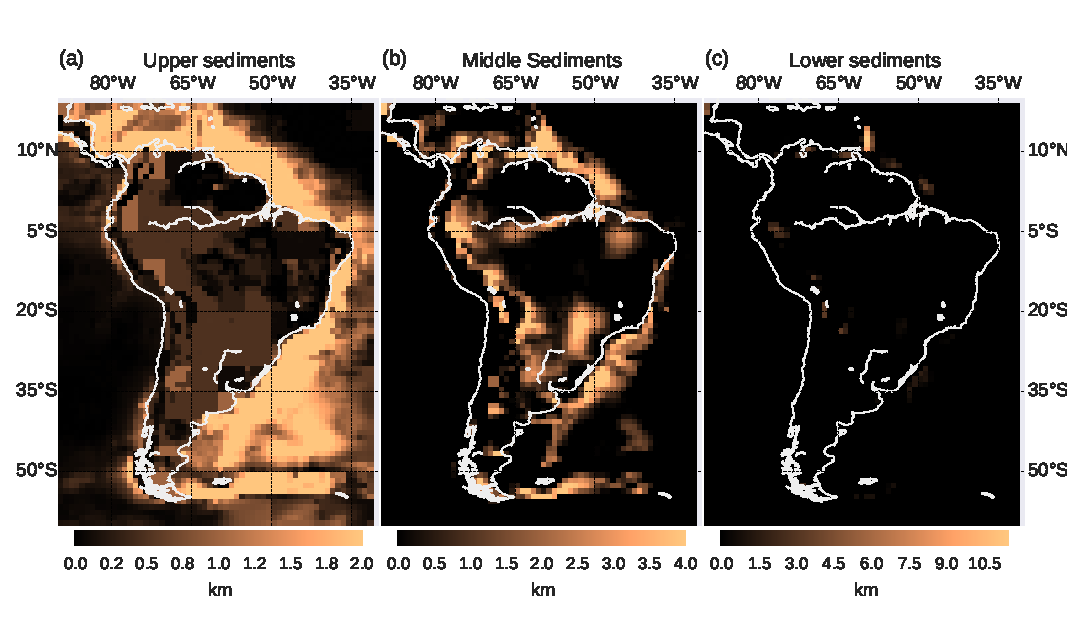
\includegraphics[width=\textwidth]{figures/paper/sam-gravity-sed}
    \caption{This is a figure caption.}
    \label{fig:sam-sed}
\end{figure*}

Fig.~\ref{fig:sam-data}.

%%%%%%%%%%%%%%%%%%%%%%%%%%%%%%%%%%%%%%%%%%%%%%%%%%%%%%%%%%%%%%%%%%%%%%%%%%%%%%%
\section{Discussion}

Meh.

%%%%%%%%%%%%%%%%%%%%%%%%%%%%%%%%%%%%%%%%%%%%%%%%%%%%%%%%%%%%%%%%%%%%%%%%%%%%%%%
\section{Conclusions}

Meh.

%%%%%%%%%%%%%%%%%%%%%%%%%%%%%%%%%%%%%%%%%%%%%%%%%%%%%%%%%%%%%%%%%%%%%%%%%%%%%%%
\section{Acknowledgments}

Meh.

\bibliographystyle{gji}
\bibliography{biblio}

\end{document}
